%!TEX root = ../thesis.tex
%*******************************************************************************
%*********************************** First Chapter *****************************
%*******************************************************************************

\chapter{Introduction}  %Title of the First Chapter

\ifpdf
    \graphicspath{{Chapter1/Figs/Raster/}{Chapter1/Figs/PDF/}{Chapter1/Figs/}}
\else
    \graphicspath{{Chapter1/Figs/Vector/}{Chapter1/Figs/}{Chapter1/Figures/}}
\fi


%********************************** %First Section  **************************************
\textit{Probabilistic Inference for Learning Control} or PILCO \citep{deisenroth2011pilco} is a model-based indirect policy search method for continuous state and action dynamical systems. PILCO evaluates a particular \textit{policy} by assuming that the distribution over inputs is Gaussian and propagating that distribution through its probabilistic representation of the transition dynamics under a particular policy. In doing so, it gains insight into the variety of states that could be visited under that policy and is able to make inferences about how effective the policy is at achieving low cost. However, this approach only allows PILCO to make decisions based on the total uncertainty as quantified by the models predictive distribution, when in fact there are two sources of uncertainty present in the system: \textit{aleatoric} and \textit{epistemic}. Aleatoric uncertainty is uncertainty due to unknowns that differ each time an agent encounters the environment (such as measurement noise) and is irreducible. Epistemic uncertainty arises from information that the agent could know in principle but currently does not, and can be reduced by observing more data. In model-based reinforcement learning, epistemic uncertainty is due to uncertainty about the model parameters. This means that in some situations PILCO could be exploring regions in the state space that are irrelevant for the task of learning control because it is making decisions based on the total uncertainty without knowledge of its constituents. In this case it could be targeting areas of high aleatoric uncertainty which could prohibit learning. 

In this dissertation I investigate how PILCO uses uncertainty in its decision making process. In particular, I disentangle and quantify the different sources of uncertainty in the model of the transition function under a given policy. PILCO is a direct policy search method and is formulated so that the \textit{cost function} is consulted directly; therefore, I examine the influence of the transition function uncertainty on cost uncertainty. I use variance as a metric for uncertainty and employ the law of total variance to decompose the total cost uncertainty into its constituents. I introduce a gold-standard Monte-Carlo scheme to separately estimate the aleatoric and epistemic uncertainties in the cost by propagating trajectories through an approximation to PILCO's dynamics model. Finally, I show that when PILCO is learning efficiently it is selecting policies associated with a high ratio of epistemic cost uncertainty to total cost uncertainty.

The aim of this dissertation is to lay the foundations for an active-exploration scheme to complement PILCO. In this dissertation I make the following contributions:
\begin{itemize}
    \item Present a variance decomposition that disentangles the sources of uncertainty in the model's predictive distribution that influence PILCO's cost under a particular policy $\pi$.
    \item Create a gold-standard Monte Carlo scheme that separates the two sources of uncertainty and quantifies them.
    \item Show that when PILCO is learning efficiently, it is selecting policies that correspond to a high ratio of epistemic cost uncertainty to total cost uncertainty. 
    \item Provide well documented code to reproduce all the results in this dissertation (see Appendix \ref{A:code}).
\end{itemize}

\section{Background} %Section - 1.1 
\label{S:background}
\textit{Reinforcement learning} is a general sequential decision making framework that is best described as learning a mapping from situations to actions in an attempt to maximise a numerical reward signal. The agent, or learner, is not told what to do and so must embark on a mission of trial-and-error to discover actions that produce the most reward. In many cases, the action taken not only influences the instantaneous reward but also the next situation or state, and therefore, all future rewards as a consequence. To find a set of optimal actions given a sequence of situations, the agent must then take into account the effect of an action on all future rewards. These two ideas; trial-and-error search and delayed reward, are the two most distinguishing features of reinforcement learning \citep{sutton2018reinforcement}.

Another highly influential idea is the trade-off between \textit{exploration} and \textit{exploitation}. For an agent to maximise the long-term reward it must favour actions which it has previously tried and found to be successful in yielding high reward. However, in order to discover those actions, it must first have tried actions that it had not previously selected. The agent must \textit{exploit} its current knowledge of the system to gain a high reward but also \textit{explore} new strategies to improve its \textit{policy}. A dilemma arises in that exclusively executing either approach will lead to a failed task. The agent must interchangeably try both approaches and progressively tend towards actions that prove to be better at attaining high reward.

There are two main approaches to reinforcement learning; \textit{model-based} and \textit{model-free} methods. Model-free methods are explicit trial-and-error learners and directly use the experience they gain through interactions with an environment to make decisions. In contrast, model-based techniques use experience indirectly by building a model of the state transition dynamics and reward structure of the environment, and evaluate actions by searching this model \citep{glascher2010states}. Model-free methods are therefore said to rely on \textit{learning} whilst model-based methods primarily  rely on \textit{planning} \citep{sutton2018reinforcement}. 

Recently, model-free methods have achieved impressive performance in a range of complex tasks such as playing Atari games, receiving only pixels and game scores as inputs \citep{mnih2015human}. These methods, however, typically require millions of interactions with the environment before they achieve reasonable performance levels. The large number of required interactions can prohibit the use of these algorithms in some domains; such as mechanical systems with components that quickly wear out \citep{deisenroth2011pilco} or safety-critical systems where carrying out many field trials is prohibitively expensive. With computational power increasing exponentially, the primary bottleneck in the deployment of real-world reinforcement learning applications is fast becoming the number of interactions with the environment \citep{Wan2018ModelbasedRL}.

Model-based methods use field trials to create a belief about the underlying environment. There are several advantages to this approach, amongst others; the learning process can be more sample-efficient \citep{deisenroth2013gaussian}, prior knowledge and experience can be integrated more easily (particularly when Bayesian models are used) \citep{lopes2012exploration}, and more recently the incorporation of \textit{counterfactual} reasoning (making inferences about actions that were not actually taken) which can be complex to implement without an explicit model-based representation of the environment \citep{buesing2018woulda}. Model-based methods are, however, not without their challenges, building accurate representations of complex real-world environments is difficult and failing to do so can lead to highly suboptimal algorithm behaviour.

Until recently, model-based techniques had not been widely applied to real-world systems. One of the main reasons for this is they can suffer from model bias. This happens when, given a data set of observed state transitions, the learned model incorrectly assumes that it fully describes the environment, when in fact there are many plausible functions that could have generated the data (\cite{atkeson1997comparison}; \cite{schneider1997exploiting}). This is demonstrated in Fig \ref{Fig:model-bias} where a small data set of transitions are observed (left panel) and several transition functions exist that could have generated the data (centre panel). Selecting any single transition function can have severe consequences because predictions are then arbitrary at positions away from the data, but are claimed with full confidence \citep{deisenroth2011pilco}. 

PILCO \citep{deisenroth2011pilco} is a model-based indirect policy search method for continuous state and action dynamical systems. PILCO learns a probabilistic Bayesian representation of the dynamical systems it seeks to govern. Bayesian models explicitly quantify their uncertainty, and PILCO uses this information in a principled way to reduce model bias by explicitly incorporating model uncertainty into long-term planning. Fig \ref{Fig:model-bias} (right panel) shows how PILCO represents the observed data by placing a posterior distribution over the transition function. 

PILCO reports unprecedented data-efficiency for a variety of control tasks, such as the cart-pole and cart-double-pole problems. Surprisingly, it does so without any intentional exploration i.e. it is \textit{greedy}. Any exploration that does occur comes from one of three sources: first, the presence of stochasticity in the system; second, the use of a saturating cost function resulting in the controller favouring uncertain states \citep{deisenroth2013gaussian}; third, future controllers being informed of the performance of past controllers. 

\begin{figure}
\centering    
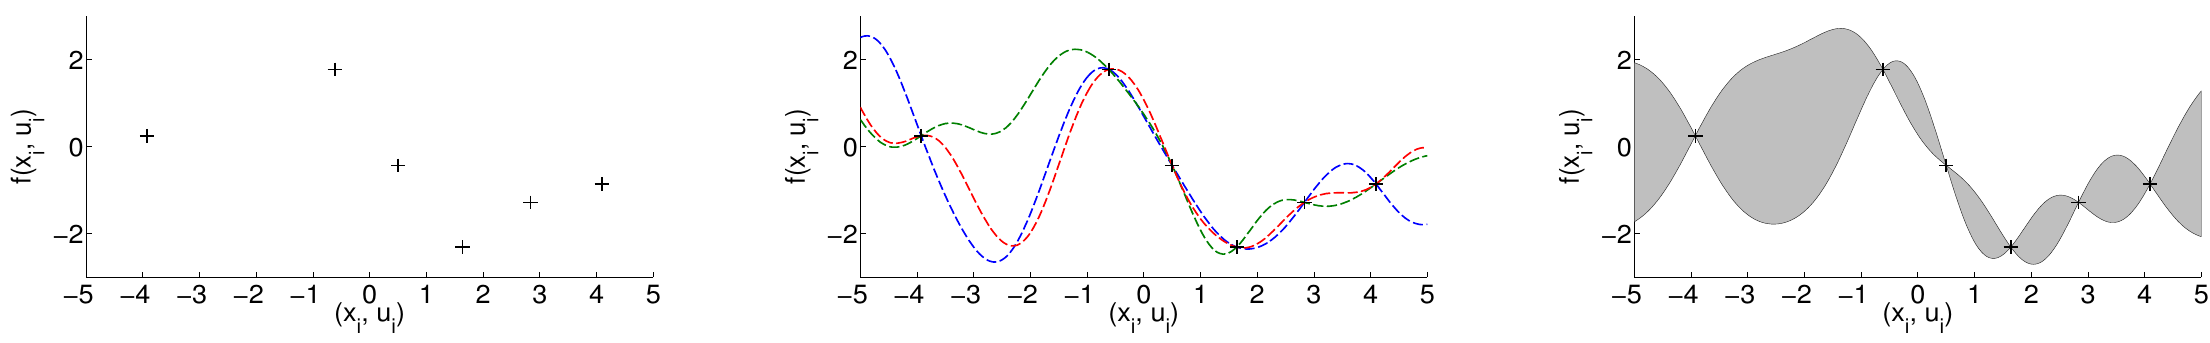
\includegraphics[width=1.0\textwidth]{Chapter1/Figures/PILCO-model-bias.png}
\caption[Model-based bias in reinforcement learning]{Small data set of observed state transitions (left). Several plausible functions that could have generated the data (centre). Posterior distribution showing model uncertainty (right). Reproduced from \citep{deisenroth2011pilco}.}
\label{Fig:model-bias}
\end{figure}

Attempting to further increase PILCO's data-efficiency would require either more informative prior knowledge of the task or extracting more relevant information from the available data. The addition of a exploration scheme would constitute the latter. Many approaches to learning control realise exploration through introducing randomness into action selection. Some approaches comprise a \textit{random exploration phase}, where the controller generates actions randomly, followed by an \textit{exploitation phase}  \citep{thrun1992active}. However, with this strategy once the exploration phase has finished, the agent is unable to adapt to environmental changes during the purely exploitative phase. Others use $\epsilon$-\textit{greedy} policies, which exploit the action with the maximum expected reward most of the time, but with some probability $\epsilon$ a random action is selected \citep{sutton2018reinforcement}. While $\epsilon$-\textit{greedy} approaches encourage learning, for real-world systems, selecting random actions can repeatedly steer the system towards undesirable or dangerous states. In addition, random action selection can be inefficient and often causes the agent to repeatedly return to already well-explored regions of the state-space because exploration is \textit{undirected}.

\textit{Information-directed} or \textit{active} exploration schemes aim to overcome the inefficiencies and risks associated with undirected exploration by driving exploration towards promising states \citep{zhaohan2019directed}. Since PILCO is primarily designed for learning control of mechanical dynamical systems, it is natural to consider this class of exploration algorithm when attempting to further improve its efficiency. Furthermore, since PILCO already quantifies model uncertainty and uses this uncertainty in long-term planning, it is also logical to attempt to incorporate this information in any considered exploration strategies. 

Currently, PILCO evaluates a particular policy by cascading uncertain inputs through the probabilistic model of the transition dynamics. In doing so, it gains insight into the variety of states that could be visited under that policy and is able to make an informed decision about how effective the policy is at achieving low cost. However, this approach only allows PILCO to make decisions based on the total uncertainty as quantified by the model, when in fact there are two sources of uncertainty present in the system. One source of uncertainty is \textit{aleatoric}; that is, representative of unknowns that differ each time the agent encounters the environment. Examples include measurement error or chaotic motion in dynamical systems that lead to stochastic transitions. The second source of uncertainty is \textit{epistemic}; that is, arising from information that the agent could know in principle but currently does not. In model-based methods, this can be thought of as lack of knowledge about the system's transition dynamics. Hence, epistemic uncertainty can be reduced by observing more data while aleatoric uncertainty is irreducible. This means that in certain situations PILCO could be making decisions based on uncertainty of which the primary constituent is aleatory. In this case, PILCO could be repeatedly selecting policies corresponding to trajectories associated with high aleatoric uncertainty which could be prohibitive to learning.

This dissertation attempts to disentangle and quantify the different sources of uncertainty (aleatoric and epistemic) present in the model of the transition function. Since PILCO is a direct policy search method, the \textit{cost function} is consulted directly, therefore, the influence of the uncertainty in the transition function on the uncertainty in the cost is examined. This is done by using variance as a metric to quantify uncertainty and employing the law of total variance to decompose the total model uncertainty into its constituents. The uncertainties are then estimated, establishing a "gold-standard" Monte-Carlo scheme that propagates trajectories through PILCO's dynamics model. The intention of the research is to lay the foundations for an active-exploration scheme to complement PILCO. 

                             % first letter S is for subscripts

%********************************** %Second Section  *************************************
\section{Related Work} %Section - 1.2
\label{S:related-work}
The use of uncertainty for exploration in reinforcement learning is well-studied, either to improve sample efficiency \citep{schneider1997exploiting} \citep{jung2010gaussian} \citep{deisenroth2011pilco} or avoid worst-case scenarios and mitigate model bias \citep{bagnell2001solving} \citep{nilim2005robust} \citep{kahn2017uncertainty} \citep{deisenroth2013gaussian}. While the majority of prior work focuses on estimation methods for either aleatoric or epistemic uncertainty, there has recently been increasing interest in \textit{decomposing} total uncertainty into these two components, which can be used independently in the decision making process.

Prior work that estimates aleatoric uncertainty, or aleatoric risk, has focused on both the randomness in the environment and the agent's actions which lead to stochastic returns. \citet{tamar2016learning} extend temporal difference methods to estimate the variance of the reward distribution by jointly estimating the second moment of the reward-to-go and the value function with a linear function approximator. The authors then derive a relationship between the two estimates to quantify risk. \citet{prashanth2013actor} define variance measures for policies to get risk-sensitive criteria for optimisation which are used alongside actor-critic gradient estimators. Other attempts at creating risk-sensitive agents include the development of distributional reinforcement learning methods which approximate the entire distribution of returns. \citet{morimura2010nonparametric} extend the Bellman equations to include the cumulative return distribution and propose an algorithm that leads to a risk-sensitive reinforcement learning paradigm. \citet{bellemare2017distributional} argue the fundamental importance of the value distribution in reinforcement learning and present theoretical results in both the policy evaluation and control settings. 

Several methods for estimating the epistemic uncertainty have been proposed. \citet{azizzadenesheli2018efficient} and \citet{lipton2018bbq} both present exploration schemes that take into account the epistemic uncertainty by performing Bayesian inference over the parameters that define the value function. \citet{pearce2018bayesian}   estimate parameter uncertainty by regularising the parameters of an ensemble of neural networks about their initialisation values, instead of zero,  and use these estimates to govern the exploration-exploitation process, resulting in steadier, more stable learning. \citet{bellemare2016unifying} take inspiration from the intrinsic motivation literature and quantify the uncertainty of an agent's knowledge through the use of density models. The authors present an algorithm for deriving a pseudo-count of state visits from an arbitrary density model which generalises count-based exploration algorithms to the non-tabular case. Finally, \citet{gal2016dropout} use Bayesian drop-out as an uncertainty estimate and provide a quantitative assessment of model uncertainty in the setting of reinforcement learning.

In the literature, a number of papers tackle the problem of producing estimates for both the aleatoric and epistemic uncertainties. \citet{clements2019estimating} build on the work of \cite{gal2016dropout} and \citet{pearce2018bayesian} and show that the disagreement between only two neural networks is sufficient to produce a low-variance estimate of the epistemic uncertainty on the return distribution and estimate aleatoric risk through a distributional framework. \citet{moerland2017efficient} uses Bayesian drop-out to estimate epistemic uncertainty and aleatoric uncertainty by propagating the return uncertainty through the Bellman equation as a Gaussian distribution. 

There are also a number of papers that consider both kinds of uncertainties in model-based reinforcement learning. \citet{chua2018deep} propose a  probabilistic ensembles with trajectory sampling (PETS) algorithm that combines uncertainty-aware deep network dynamics models with sampling-based uncertainty propagation which has the ability to isolate both sources of uncertainty. Finally, \cite{depeweg2017decomposition} present two uncertainty decompositions for Bayesian neural network models with latent variables that isolate both sources of uncertainty. The first is in the form a variance decomposition and is similar to what is presented in this work and the second in terms of mutual information. The sources of uncertainty are then related to risk-sensitive reinforcement learning.